% LaTeX source for joint paper on SUNDIALS
% Version of 18 August 2003

\documentclass[acmtoms]{acmtrans2m}
\usepackage{amsmath, amssymb}
\usepackage{epsfig}
\usepackage{tabularx}
%\usepackage{showlabels}

\newcommand{\dfdy}{\frac{\partial f}{\partial y}}
\newcommand{\dfdyI}{\partial f / \partial y}
\newcommand{\dfdpi}{\frac{\partial f}{\partial p_i}}
\newcommand{\dfdpiI}{\partial f / \partial p_i}

\newcommand{\mb}[1]{{\mbox{\scriptsize #1}}}

\makeatletter
\newcommand{\figcaption}{\def\@captype{figure}\caption}
\newcommand{\tabcaption}{\def\@captype{table}\caption}
\makeatother

\acmVolume{V}
\acmNumber{N}
\acmYear{Y}
\acmMonth{Month}

\markboth{R. Serban and A.C. Hindmarsh}
{CVODES: An ODE solver with sensitivity analysis capabilities}

\title{CVODES: An ODE solver with sensitivity analysis capabilities}

\author{RADU SERBAN and ALAN C. HINDMARSH \\
  Center for Applied Scientific Computing \\
  Lawrence Livermore National Laboratory}

\begin{abstract}
CVODES, which is part of the SUNDIALS software suite,
is a stiff and nonstiff ordinary differential equation initial 
value problem solver with sensitivity analysis capabilities. 
CVODES is written in a data-independent manner, with a highly 
modular structure to allow incorporation of different 
preconditioning and/or linear solver methods. It shares with the 
other SUNDIALS solvers several common modules, most notably the 
generic kernel of vector operations and a set of generic linear 
solvers and preconditioners.

CVODES solves the IVP by one of two methods -- backward differentiation 
formula or Adams-Moulton -- both implemented in a variable-step, 
variable-order form. The forward sensitivity module in CVODES implements 
the simultaneous corrector method, as well as two flavors of 
staggered corrector methods. Its adjoint sensitivity module 
provides a combination of checkpointing and cubic Hermite interpolation 
for the efficient generation of the forward solution during the adjoint 
system integration.

We describe the current capabilities of CVODES, its design principles,
and its user interface.  We also give an example problem to illustrate
the performance of CVODES.

\end{abstract}

\category{G.4}{Mathematical Software}{Algorithm design and analysis}

\category{G.1.7}{Numerical Analysis}{Ordinary Differential Equations}
[Initial value problems \and Multistep methods \and Stiff equations]

%\category{G.1.m}{Miscellaneous}{Sensitivity Analysis}
%[Forward methods \and Adjoint methods]

\terms{Algorithms, Design}

\keywords{ODEs, Forward Sensitivity Analysis, Adjoint Sensitivity Analysis}

%=======================================================================

\begin{document}

\setcounter{page}{1}

\begin{bottomstuff}
Authors' address: 
Radu Serban, 
Lawrence Livermore National Laboratory, P.O. Box 808, L-560,
Livermore, CA 94551; email: {\tt radu@llnl.gov};
Alan C. Hindmarsh,
Lawrence Livermore National Laboratory, P.O. Box 808, L-560,
Livermore, CA 94551; email: {\tt alanh@llnl.gov};
\newline
This work was performed under the auspices of the
U.S. Department of Energy by the University of California,
Lawrence Livermore National Laboratory, under contract No.
W-7405-Eng-48.
\end{bottomstuff}

\maketitle

%=======================================================================
% Include sections

\section{Introduction}

With the ever-increasing capabilities of modern computers, simulation
code developers are challenged to develop fast and robust software
capable of solving problems with increasingly higher resolutions and
modeling more complex
physical phenomena.  At the heart of many numerical simulation codes
lie systems of nonlinear algebraic or time-dependent equations, and
simulation scientists continue to require efficient solvers for these
systems.

To meet this need, Lawrence Livermore National Laboratory
has a long history of research and development in ordinary
differential equation (ODE) methods and software, as well as closely related
areas, with emphasis on applications to partial differential equations
(PDEs).  Among the popular Fortran 77 solvers written at LLNL are the
following:
\begin{itemize}
\item VODE: a solver for ODE initial-value problems for stiff/nonstiff
systems, with direct solution of linear systems, by Brown, Byrne, and
Hindmarsh \cite{BBH:89}.
\item VODPK: a variant of VODE with preconditioned Krylov (GMRES
iteration \cite{SaSc:86}) solution of the linear systems in place
of direct methods, by Brown, Byrne, and Hindmarsh \cite{Byr:92}.
\item NKSOL: a Newton-Krylov (GMRES) solver for nonlinear algebraic
systems, by Brown and Saad \cite{BrSa:90}.
\item DASPK: a solver for differential-algebraic equation (DAE)
systems (a variant of DASSL) with both direct and preconditioned
Krylov solution methods for the linear systems, by Brown, Hindmarsh,
and Petzold \cite{BHP:94}.
\end{itemize}
Starting in 1993, the push to solve large systems in parallel
motivated work to write or rewrite solvers in C. Moving to the C
language was done to: exploit features of C not present in Fortran
77 while using languages with stable compilers (F90/95 were not
yet stable when this work started); achieve a more object-oriented
design; facilitate the use of the codes with other object-oriented
codes being written in C and C++; maximize the reuse of code
modules; and facilitate the extension from a serial to a parallel
implementation. The first result of the C effort was CVODE. This
code was a rewrite in ANSI standard C of the VODE and VODPK
solvers combined, for serial machines \cite{CoHi:94,CoHi:96}.  The
next result of this effort was PVODE, a parallel extension of
CVODE \cite{ByHi:98,ByHi:99}. Similar rewrites of NKSOL and DASPK
followed, using the same general design as CVODE and PVODE.  The
resulting solvers are called KINSOL and IDA, respectively. More
recently, we have merged the PVODE and CVODE codes into a single
solver, CVODE.

The main numerical operations performed in these codes are
operations on data vectors, and the codes have been written in
terms of interfaces to these vector operations.  The result of
this design is that users can relatively easily provide their own
data structures to the solvers by telling the solver about their
structures and providing the required operations on them. The
codes also come with default vector structures
with pre-defined operation implementations for both serial and
distributed memory parallel environments in case a user prefers to
not supply their own structures. In addition, all parallelism is
contained within specific vector operations (norms, dot products,
etc.)  No other operations within the solvers require knowledge of
parallelism. Thus, using a solver in parallel consists of using
a parallel vector implementation, either the one provided with
SUNDIALS, or the user's own parallel vector structure, 
underneath the solver.  
Hence, we no longer make a distinction between parallel and serial 
versions of the codes.

These codes have been combined into the core of SUNDIALS, the
SUite of Nonlinear and DIfferential/Algebraic equation Solvers.
This suite, consisting of CVODE, KINSOL, and IDA (along with
current and future augmentations to include forward and adjoint
sensitivity analysis capabilities), was implemented with the goal
of providing robust time integrators and nonlinear solvers that
can easily be incorporated into existing simulation codes.  The
primary design goals were to require minimal information from the
user, allow users to easily supply their own data structures
underneath the solvers, and allow for easy incorporation of
user-supplied linear solvers and preconditioners.

As simulations have increased in size and complexity, the
relationship between computed results and problem parameters has
become harder to establish.  Scientists have a greater need to
understand answers to questions like the following.  Which model
parameters are most influential? How can parameters be adjusted to
better match experimental data? What is the uncertainty in
solutions given uncertainty in data?  Sensitivity analysis
provides information about the relationship between simulation
results and model data, which can be critical to answering these
questions. In addition, for a given parameter, sensitivities can
be computed in a modest multiple of the computing time of the
simulation itself.

SUNDIALS is being expanded to include forward and adjoint
sensitivity versions of the solvers. The first of these, CVODES,
is complete.  A brief description of the strategy for adding
sensitivity analysis in a way that respects the user interfaces of
the SUNDIALS codes is contained in this paper, and a more thorough
description of the CVODES package (which is distinct from but
built on the same core code as CVODE) is contained in a companion
paper \cite{SeHi:03}. The second sensitivity solver will be IDAS
and is currently under development. Extensions to KINSOL for
sensitivity analysis will be completed if need arises.

The rest of this paper is organized as follows.  In Section
\ref{s:basic_solvers}, the algorithms in the three core solvers of
SUNDIALS are presented. We have attempted to identify many of the
heuristics related to stopping criteria and finite-difference
parameter selection where appropriate, as these items can
sometimes affect algorithm performance significantly. In Section
\ref{s:preconditioning}, the preconditioning packages supplied
with SUNDIALS are described.  Section \ref{s:sensitivity_analysis}
overviews the CVODES package and strategies for adding sensitivity
capabilities to the codes. Sections \ref{s:organization} and
\ref{s:usage} describe the organization of the codes within the
suite and the philosophy of the user interface. Availability of
the codes is given in Section \ref{s:availability}.  Finally,
comments on applications of SUNDIALS, concluding remarks, and
indications of future development are contained in the last
section.

\section{Algorithms}\label{s:algorithms}

CVODES solves initial value problems with free parameters. 
Such problems can be stated as
\begin{equation}\label{e:ivp}
\dot{y}  = f(t,\,y,\,p) \, , \quad y(t_0)  = y_0(p) \, ,
\end{equation}
where $y \in {\bf R}^N$ is  the vector of state variables, 
$\dot{y}\,=dy/dt$, and $p \in {\bf R}^{N_p}$ are problem parameters.
Additionally, CVODES can also compute first order derivative
information, performing either
{\em forward sensitivity analysis} or {\em adjoint sensitivity analysis}.
In the first case, CVODES computes the sensitivities of the solution
with respect to the parameters $p$, while in the second case, CVODES
computes the gradient of a {\em derived function} with respect to the
parameters $p$.

In the rest of this section we describe the algorithms implemented in
CVODES, with emphasis on sensitivity analysis. We give only a brief
overview of the ODE integration algorithm to introduce some of the
quantities needed in the sequel.  Since CVODES shares its main
integration algorithm with CVODE, the interested reader is directed
to~\cite{HBGLSSW:04}.

%-------------------------------------------------------------------------------

\subsection{ODE Integration}\label{ss:integration}

CVODES solves the IVP using either Backward Differentiation Formula
(BDF) methods or Adams-Moulton methods.  Both are implemented with
dynamically varying stepsize and order, based on the control of local
errors to meet user-specified tolerances.  A central feature of the
method is the solution, at each time step, of a nonlinear system of
size $N$, of the form
\begin{equation}\label{e:nonlinear}
    F(y_n) \equiv y_n - \gamma_n f(t_n,\,y_n,\,p) - a_n = 0 \,
\end{equation}
where $\gamma_n$ is a scalar and $a_n$ is a constant vector.
This system is solved by either functional (fixpoint) iteration or
some form of Newton iteration.  In the latter case, the matrix in the
linear system for Newton corrections has the form $M = I-\gamma_nJ_n$,
where $J_n = {\partial f}/{\partial y}$ at $(t_n,y_n)$.

CVODES also incorporates an algorithm for special treatment of
quadratures depending on the solution $y$ of (\ref{e:ivp}).
An efficient quadrature computation is needed in the context of
adjoint sensitivity analysis (see Section~\ref{ss:adj_sensitivity}).
Evaluation of integrals of the form
$G = \int_{t_0}^{t_\mb{f}} g(t,y,p) dt$ can be done efficiently using the
underlying linear multistep method interpolating polynomials by
appending to (\ref{e:ivp}) an additional ODE
$\dot\phi = g(t,y,p)$, with initial condition $\phi(t_0) = 0$,
in which case $G = \phi(t_f)$. In the context of an implicit ODE
integrator, since the right-hand side of this additional equation does not
depend on $\phi$, such equations need not participate in the solution of
the nonlinear system~(\ref{e:nonlinear}). CVODES allows the user to
identify these equations separately from those in~(\ref{e:ivp}) and
provides the option of including or excluding $\phi$ from the error
control algorithm.
A similar treatment of quadratures is included in the DASPK3
code~\cite{LiPe:99a,LiPe:00}.


A complete description of the CVODES integration algorithm, including 
the nonlinear solver convergence, error control mechanism, and heuristics 
related to stopping criteria and finite-difference parameter selection, is
given in~\cite{HBGLSSW:04}.

%-------------------------------------------------------------------------------

\subsection{Forward Sensitivity Analysis}\label{ss:fwd_sensitivity}

Typically, the governing equations of complex, large-scale models
depend on various parameters,  through the right-hand side vector 
and/or through the vector of initial conditions, as in (\ref{e:ivp}).
In addition to numerically solving the ODEs, it may be desirable to
determine the sensitivity of the results with respect to the model
parameters. 
Such sensitivity information can be used to estimate which
parameters are most influential in affecting the behavior of the
simulation or to evaluate optimization gradients (in the setting of dynamic
optimization, parameter estimation, optimal control, etc.).

The {\em solution sensitivity} with respect to the model parameter
$p_i$ is defined as the vector 
$s_i (t) = {\partial y(t)}/{\partial p_i}$
and satisfies the following {\em forward sensitivity equations}
(or in short {\em sensitivity equations}):
\begin{equation}\label{e:sens_eqns}
\dot{s_i}  = \frac{\partial f}{\partial y} s_i + \frac{\partial f}{\partial p_i} \, ,
\quad s_i(t_0)  = \frac{\partial y_{0}(p)}{\partial p_i} \, ,
\end{equation}
obtained by applying the chain rule of differentiation to the original
ODEs~(\ref{e:ivp}). 

When performing forward sensitivity analysis, CVODES carries out the time integration 
of the combined system, (\ref{e:ivp}) and (\ref{e:sens_eqns}), by viewing it as an ODE
system of size $N(N_s+1)$, where $N_s$ represents a subset of model parameters $p_i$, 
with respect to which sensitivities are desired ($N_s \le N_p$). 
The sensitivity equations are solved with the same linear multistep formula that
was selected for the original ODEs and, if Newton iteration was selected, the
same linear solver is used in the correction phase for both state and sensitivity 
variables. In addition, CVODES offers the option of including
({\em full error control}) or excluding
({\em partial error control}) the sensitivity variables from the local 
error test.

\subsubsection{Forward sensitivity methods}
In what follows we briefly describe three methods that have been proposed for the 
solution of the combined ODE and sensitivity system for the vector
${\hat y} = [y, s_1, \ldots , s_{N_s}]$.

\begin{itemize}

\item[{\em Staggered Direct.}]
  In this approach \cite{CaSt:85}, the nonlinear system (\ref{e:nonlinear}) is first 
  solved and, once an acceptable numerical solution is obtained, the sensitivity 
  variables at the new step are found by directly solving (\ref{e:sens_eqns}) 
  after the BDF discretization is used to eliminate ${\dot s}_i$. 
  Although the system matrix of the above linear system is based on exactly the same 
  information as the matrix $M$, it must be updated and factored 
  at every step of the integration, in contrast to $M$ which is updated only ocasionally. 
  For problems with many parameters (relative to the problem size), the staggered direct 
  method can outperform the methods described below~\cite{LPZ:99}.
  However, the computational cost associated with matrix updates and factorizations 
  makes this method unattractive for problems with many more states than parameters
  (such as those arising from semidiscretization of PDEs).
  
\item[{\em Simultaneous Corrector.}] 
  In this method \cite{MaPe:96}, the BDF discretization is applied simultaneously
  to both the original equations (\ref{e:ivp}) and the sensitivity systems
  (\ref{e:sens_eqns}) resulting in an extended nonlinear system 
  %%   \begin{equation*}
  %%     {\hat G}({\hat y}_n) \equiv  
  %%     {\hat y}_n - h_n\beta_{n,0} {\hat f}(t_n,\,{\hat y}_n) - {\hat a}_n = 0 \, ,
  %%   \end{equation*}
  %%   where
  %%   ${\hat f} = [ f(t,y,p), \ldots , (\dfdyI)(t,y,p) s_i + (\dfdpiI)(t,y,p) , \ldots ]$
  %%   and ${\hat a}_n$ are the terms in the BDF discretization that depend on the
  %%   solution at previous integration steps.
  in the uknown ${\hat y} = [y, s_1, \ldots , s_{N_s}]$.
  This combined nonlinear system can be solved using either functional or
  Newton iteration. In the latter case, Maly and Petzold have shown
  that 2-step quadratic convergence can be attained with a modified Newton scheme
  which uses only the block-diagonal portion of the iteration matrix.
  This results in a decoupling that allows the reuse of 
  $M$ without additional matrix factorizations. However, the products
  $(\dfdyI)s_i$ as well as the vectors $\dfdpiI$ must still be reevaluated at 
  each step of the iterative process to update the 
  sensitivity portions of the residual.
  
\item[{\em Staggered corrector.}] In this approach \cite{FTB:97}, as in the staggered direct method,
  the nonlinear system (\ref{e:nonlinear}) is solved first for the state variables.
  Then, a separate nonlinear iteration is used to solve the sensitivity system.
  In this approach, the vectors $\dfdpiI$ need be updated only once per integration step, 
  after the state correction phase has converged. 
  When using functional iteration, this amounts to using a stationary iterative method for
  the linear system (\ref{e:sens_eqns}). When using Newton iteration, this amounts to 
  using a modified-Newton iteration to solve the linear system (\ref{e:sens_eqns}), 
  the Newton iteration matrix being only an approximation to the system matrix.
  An important observation is that the staggered corrector method, combined with 
  Newton iterations and the SPGMR linear solver, effectively results in a staggered direct 
  method~\cite{Toc:01}.
  Indeed, SPGMR requires only the action of the matrix $M$ on a vector and
  this can be provided with up-to-date Jacobian information. Therefore, the
  modified Newton procedure will theoretically converge 
  after one iteration.

\end{itemize}  
%%
CVODES implements the simultaneous corrector method and two flavors of the 
staggered corrector method which differ only if the sensitivity variables are
included in the error control test.
In the {\em full error control} case, 
the first variant of the staggered corrector method requires the convergence of 
the nonlinear sensitivity iterations for all $N_s$ sensitivity sytems and then 
performs the error test on the sensitivity variables. The second variant of the method
will perform the error test for each sensitivity vector $s_i$ ($i=1,\ldots,N_s$),
individually, as they pass the convergence test. Differences in performance
between the two variants may therefore be noticed whenever one of the sensitivity 
vectors $s_i$ fails a convergence or error test. 

We note that the DASPK3.0 code \cite{LiPe:99b,LiPe:99a} implements the staggered
direct, simultaneous corrector, and staggered corrector methods. The code
DSL48S \cite{FTB:97,Fee:98} also contains the staggered corrector method.

\subsubsection{Selection of the absolute tolerances for sensitivity variables}
If the sensitivities are included in the error test, CVODES provides an 
automated estimation of absolute tolerances for the sensitivity variables 
based on the absolute tolerance for the corresponding state variable.
The relative tolerance for sensitivity variables is set to be the same as for 
the state variables. The selection of absolute tolerances for the sensitivity 
variables is based on the observation that the sensitivity vector $s_i$ will have 
units of $[y]/[p_i]$.
With this, the absolute tolerance for the $j$-th component of the sensitivity
vector $s_i$ is set to ${\mbox{\sc atol}_j}/{|{\bar p}_i|}$,
where $\mbox{\sc atol}_j$ are the absolute tolerances for the state variables and $\bar p$
is a vector of scaling factors that are dimensionally consistent with
the model parameters $p$ and give indication of their order of magnitude.
This choice of relative and absolute tolerances is equivalent 
to requiring that the weighted root-mean-square norm of the sensitivity 
vector $s_i$ with weights based on $s_i$ is the same as the
weighted root-mean-square norm of the vector of scaled sensitivities 
${\bar s}_i = |{\bar p}_i| s_i$ with weights based on the state variables
(the scaled sensitivities ${\bar s}_i$ being dimensionally consistent with the
state variables).
%
However, this choice of tolerances for the $s_i$ may be a poor one, and the user 
of CVODES can provide different values as an option.

\subsubsection{Evaluation of the sensitivity right-hand side}
There are several methods for evaluating the right-hand side of the sensitivity 
systems (\ref{e:sens_eqns}): analytic evaluation, automatic differentiation, 
complex-step approximation, and finite differences (or directional derivatives).

Since it allows for user-defined functions for the evaluation of any and all 
derivative information, CVODES provides all the software hooks for implementing 
interfaces to automatic differentiation or complex-step approximation. 
We have prototyped an automated code generator tool (not included in
the CVODES distribution) which parses C code and generates C++ code to
perform complex arithmetic. The user's right-hand side function can
thus be transformed to allow for the automatic generation of
derivative information using complex-step approximations~\cite{MSA:03}.
This approach allows for very accurate numerical estimation of
derivatives as it circumvents the subtraction cancellation error
typical for finite difference methods. However, any code
transformation approach to the automatic generation of derivative
information from C functions (for example ADIC~\cite{BRM:97})
has the disadvantage of requiring transformations on the user's data
structures, which are otherwise treated as black boxes by CVODES.
This makes the design of general interfaces a challenging task, but we 
are investigating avenues to overcome this issue.

The default option in CVODES for the evaluation of sensitivity right-hand 
sides is to use finite difference-based approximations for the terms $(\dfdyI) s_i$ 
and $\dfdpiI$, or directional derivatives to evaluate
$(\dfdyI) s_i + \dfdpiI$.
As is typical for finite differences, the proper choice of perturbations is a 
delicate matter. CVODES takes into account several problem-related features:
the relative ODE error tolerance $\mbox{\sc rtol}$, the machine unit roundoff $U$,
the scale factor ${\bar p}_i$, and the weighted root-mean-square norm of the 
sensitivity vector $s_i$.

Using central finite differences as an example, the two terms 
$({\partial f}/{\partial y}) s_i$ 
and ${\partial f}/{\partial p_i}$ in the right-hand side of (\ref{e:sens_eqns})
can be evaluated separately:
\begin{gather}
  \frac{\partial f}{\partial y} s_i \approx \frac{f(t, y+\sigma_y s_i, p)-
    f(t, y-\sigma_y s_i, p)}{2\,\sigma_y} \, , \label{e:fd2} \\
  \frac{\partial f}{\partial p_i} \approx \frac{f(t,y,p + \sigma_i e_i)-
    f(t,y,p - \sigma_i e_i)}{2\,\sigma_i} \, , \tag{\ref{e:fd2}'} \\
  \sigma_i = |{\bar p}_i| \sqrt{\max( \mbox{\sc rtol} , U)} \, , \quad
  \sigma_y = \frac{1}{\max(1/\sigma_i, \|s_i\|_{\mbox{\scriptsize WRMS}}
                                          /|{\bar p}_i|)} \, , \nonumber
\end{gather}
simultaneously:
\begin{gather}
  \frac{\partial f}{\partial y} s_i + \frac{\partial f}{\partial p_i} \approx
  \frac{f(t, y+\sigma s_i, p + \sigma e_i) -
    f(t, y-\sigma s_i, p - \sigma e_i)}{2\,\sigma} \, , \label{e:dd2} \\
  \sigma = \min(\sigma_i, \sigma_y) \, , \nonumber
\end{gather}
or adaptively switching between (\ref{e:fd2})+(\ref{e:fd2}') and (\ref{e:dd2}), 
depending on the relative size of the estimated finite difference 
increments $\sigma_i$ and $\sigma_y$.

%-------------------------------------------------------------------------------

\subsection{Adjoint Sensitivity Analysis}\label{ss:adj_sensitivity}

In the {\em forward sensitivity approach} described in the previous
section, obtaining sensitivities with respect to $N_s$ parameters is roughly
equivalent to solving an ODE system of size $(1+N_s) N$. This can become 
prohibitively expensive, especially for large-scale problems, if sensitivities
with respect to many parameters are desired.
In this situation, the {\em adjoint sensitivity method} is a very
attractive alternative, provided that we do not need the solution sensitivities
$s_i$, but rather the gradients with respect to model parameters of a relatively 
few derived functionals of the solution. In other words, if $y(t)$ is the solution
of (\ref{e:ivp}), we wish to evaluate the gradient ${dG}/{dp}$ of
\begin{equation}\label{e:G}
G(p) = \int_{t_0}^{t_\mb{f}} g(t, y, p) dt \, ,
\end{equation}
or, alternatively, the gradient ${dg}/{dp}$ of the function $g(t, x, p)$ 
at time $t_\mb{f}$. 
The function $g$ must be smooth enough that $\partial g / \partial y$ 
and $\partial g / \partial p$ exist and are bounded. 
%
The gradient of $G$ with respect to $p$ is simply
\begin{equation}\label{e:dGdp}
  \frac{dG}{dp} = \lambda^T(t_0) s(t_0) + 
  \int_{t_0}^{t_\mb{f}} \left( \frac{\partial g}{\partial p} + 
    \lambda^T \frac{\partial f}{\partial p} \right) dt,
\end{equation}
where $\lambda$ is solution of
\begin{equation}\label{e:adj_eqns}
{\dot \lambda} = -\left( \dfdy \right)^T \lambda - 
\left( \frac{\partial g}{\partial y} \right)^T \, ,
\quad \lambda(t_\mb{f}) = 0
\end{equation}
and $s(t_0) = \partial y_0 / \partial p$.
%
The gradient of $g(t_\mb{f},y,p)$ with respect to $p$ can be then obtained
by using the Leibnitz differentiation rule \cite{CLPS:03}.

The first thing to notice about the adjoint system (\ref{e:adj_eqns})
is that there is no explicit specification of the parameters $p$; this
implies that, once the solution $\lambda$ is found, the formula
(\ref{e:dGdp}) can then be used to find the gradient of $G$ with
respect to any of the parameters $p$.
The second important remark is that the adjoint systems are terminal
value problems which depend on the solution $y(t)$ of the original IVP
(\ref{e:ivp}).  Therefore, a procedure is needed for providing the
states $y$ obtained during a forward integration phase of
(\ref{e:ivp}) to CVODES during the backward integration phase of
(\ref{e:adj_eqns}).
The approach adopted in CVODES, similar to that implemented
in DASPKADJOINT \cite{LiPe:00}, is justified below.

Since CVODES implements variable-stepsize integration formulas,
it is unlikely that the states will be available at the desired time and
therefore some form of interpolation is needed. The CVODES implementation
being also variable-order, it is possible that during the forward
integration phase the order may be reduced as low as first order,
which means that there may be points in time where only $y$ and ${\dot y}$
are available. Therefore, CVODES employs a cubic Hermite interpolation
algorithm. However, especially for large-scale problems and long integration
intervals, the number and size of the vectors $y$ and ${\dot y}$ that would 
need to be stored make this approach computationally intractable. 

CVODES settles for a compromise between storage space and execution
time by implementing a check-pointing scheme which, at the cost of at
most one additional forward integration, offers the best possible
estimate of memory requirements for adjoint sensitivity analysis.
Note that truly optimal checkpointing \cite{GrWa:00} cannot be used
since the number of integration steps is not known apriori.

%% To begin with,
%% based on the problem size $N$ and the available memory, the user decides on 
%% the number $N_d$ of data pairs ($y$, ${\dot y}$) that can be kept in memory for 
%% the purpose of interpolation. Then, during the first forward integration stage, 
%% every $N_d$ integration steps a check point is formed by saving enough information
%% (either in memory or on disk if needed) to allow for a hot restart, that is, a restart
%% that will exactly reproduce the forward integration. In order to avoid storing
%% Jacobian-related data at each check point, a reevaluation of the iteration matrix
%% is forced before each check point.
%% The backward integration from check point $i+1$ to check point $i$ is preceded
%% by a forward integration from $i$ to $i+1$ during which $N_d$ data pairs 
%% ($y$, ${\dot y}$) are generated and stored in memory for interpolation.
%% This procedure is illustrated in Fig.~\ref{f:ckpnt}.
%
\begin{figure}
\centerline{\psfig{figure=ckpnt.eps,width=4in}}
\caption {Illustration of the check-pointing algorithm for generation of 
  the forward solution during the integration of the adjoint system.}
\label{f:ckpnt}
\end{figure}
%%
This approach, illustrated in Fig.~\ref{f:ckpnt}, transfers the uncertainty in the number of integration
steps in the forward integration phase to uncertainty in the final number of check 
points. However, $N_c$ is much smaller than the number of steps taken during
the forward integration, and there is no major penalty for writing and then reading
check point data to/from a temporary file.
%

We note that the adjoint sensitivity module in CVODES provides the 
infrastructure to integrate backwards in time any ODE terminal value problem
dependent on the solution of the IVP (\ref{e:ivp}), including
the adjoint system (\ref{e:adj_eqns}), as well as any other
quadrature ODEs that may be needed in evaluating the integral in (\ref{e:dGdp}).
In particular, for ODE systems arising from semi-discretization
of time-dependent PDEs, this feature allows for integration either of the 
discretized adjoint PDE system or of the adjoint of the discretized PDE,
since these two formulations are not equivalent~\cite{ArSa:97,LiPe:04}.

Finally, we mention that, when using the backward integration module for adjoint
sensitivity analysis, the CVODES interface allows for user-provided
functions for the evaluation of the adjoint systems that are generated through
reverse automatic differentiation. Due to the current development stage of
reverse AD tools for C codes, CVODES cannot provide generic wrappers
(as done, for example, in DASPKADJOINT for Fortran77 codes). At this time, the
burden of interfacing CVODE with AD-generated functions must rely on
the user.

\section{Code Organization}
\label{s:organization}

The writing of CVODE from the Fortran 77 solvers VODE and VODPK
initiated a complete redesign and reorganization of the existing
LLNL solver coding. The features of the design of CVODE include
the following:
\begin{itemize}
\item Memory allocation is heavily used.
\item The linear solver modules are separate from the core integrator,
so that the latter is independent of the method for solving linear
systems.
\item Each linear solver module contains  a generic solver, which is
independent of the ODE context, together with an interface to the CVODE core
integrator module.
\item The vector operations  (linear sums, dot products, norms, etc.) on
$N$-vectors are isolated in a separate NVECTOR module.
\end{itemize}

The process of modularization has continued with the development of CVODE,
KINSOL, and IDA. The SUNDIALS distribution now contains a number of common
modules in a shared directory. Additionally, compilation of SUNDIALS is now
independent of any prior specification of a particular NVECTOR
implementation, facilitating the use of binary libraries. The current
NVECTOR design also allows the use of multiple implementations within the
same code, as may be required to meet user needs.

Figure \ref{fig-sunorg} shows the overall structure of SUNDIALS, with the
various separate modules. The evolution of SUNDIALS has been directed toward
keeping the entire set of solvers in mind. Thus, CVODE, KINSOL, and IDA share
much in their organization and have a number of common modules.  The
separation of the linear solvers from the core integrators allows for easy
addition of linear solvers not currently included in SUNDIALS. At the bottom
level is the NVECTOR module, providing key vector operations such as creation,
duplication, destruction, summation, and dot products on potentially
distributed data vectors. Serial and parallel NVECTOR implementations are
included with SUNDIALS, but a user can substitute his/her own implementation
as useful. Two small modules defining several data types and elementary
mathematical operations are also included.

\begin{figure}[tp]
\centerline{\psfig{figure=sunorg.eps,width=\textwidth}}
\caption{Overall structure of the SUNDIALS  package.}
\label{fig-sunorg}
\end{figure}

A number of necessary and optional user-supplied routines for the solvers
in SUNDIALS
are not shown in \mbox{Figure \ref{fig-sunorg}}. The user must
provide a routine for the evaluation of $f$ (CVODE) or $F$ (KINSOL and
IDA). The user-provided routines may include, depending on the options
chosen, routines for Jacobian evaluation (direct cases) or Jacobian-vector
products (Krylov case), and routines for the setup and solution of Krylov
preconditioners.


\subsection{Shared Modules - Linear Solvers}

As can be seen in \mbox{Figure \ref{fig-sunorg}}, three linear solver
packages are currently included with SUNDIALS: a direct dense matrix solver
(DENSE); a direct band solver (BAND); and an iterative Krylov solver
(SPGMR). These are stand-alone packages in their own right.

The shared linear solvers are accessed from SUNDIALS via solver-specific
wrappers.  Thus, SPGMR is accessed via CVSPGMR, IDASPGMR, and KINSPGMR,
for CVODE (and CVODES), IDA, and KINSOL, respectively. For the DENSE
solver, the wrappers are CVDENSE and IDADENSE for CVODE/CVODES and
IDA, respectively. Similar wrappers for BAND are CVBAND and IDABAND.

Within each solver, each linear solver module consists primarily of the
user-callable function that specifies that linear solver, and four or five
wrapper routines.  The wrappers conform to a fixed set of specifications,
enabling the central solver routines to be independent of the linear
system method used.  Specifically, for each such module, there are
four wrappers --- for initialization, Jacobian/precondioner matrix
setup, linear system solution, and memory freeing.  The IDA modules
have a fifth wrapper, for linear solver performance monitoring.  These
wrapper specifications are fully described in the user documentation
for each solver.  By following those, and using any of the existing modules
as a model, the user can add a linear solver module to the package, if
appropriate.

\subsection{Shared Modules - NVECTOR}

A generic NVECTOR implementation is used within SUNDIALS to
operate on vectors. This generic implementation defines an NVECTOR
structure which consists of an implementation-specific content and a set 
of abstract vector operations. The NVECTOR module also provides a set of 
wrappers for accessing the actual vector operations of the implementation 
under which an NVECTOR was created. 
Because details of vector operations are thus encapsulated within each specific
NVECTOR implementation, the solvers in SUNDIALS are now independent of a specific
implementation. This allows the solvers to be precompiled as binary
libraries and allows more than one NVECTOR implementation to be used within
a single program.

A particular NVECTOR implementation, such as the serial and parallel
implementations included with SUNDIALS or a user-provided implementation,
must provide certain functionalities. 
At a minimum, each implementation must provide functions to create a new
vector, a function to destroy such vectors, and the definitions of
vector operations required by the SUNDIALS solvers, including, for example, 
duplication, summation, element-by-element inversion, and dot product. 

If neither the serial nor parallel NVECTOR implementation provided within
SUNDIALS is suitable, the user can provide one or more NVECTOR implementations.  
For example, it might (and has been) more practical to substitute a more complex
data structure in a parallel implementation.

For complete details, see the user documentation for any of the solvers in 
SUNDIALS~\cite{HiSe:04cvode,HiSe:04cvodes,HiSe:04ida,HSW:04kinsol}.

\subsection{User Interface Design}

When CVODE was initially developed from VODE and VODPK, its user
interface was completely redesigned, and the same design principles
were adopted when the other solvers were added to the suite.  Further
changes in the interface design were made more recently.  Unlike the
typical Fortran solver, where the interface consists of one callable
routine with many arguments, the user interface to each of the
SUNDIALS solvers involves many callable routines, each with only a few
arguments.  The various routines specify the various aspects of the
problem to be solved and of the solution method to be used, or
retrieve information about the solution.  For each solver, there are
separate (required) calls that initialize and allocate memory for
the problem solver and for the linear system solver it will use.  
Then there are optional calls to specify various
optional inputs (ranging from scalars like maximum method order to the
user-supplied Jacobian routine), and optional calls to obtain optional
outputs (mostly performance statistics).  Finally, there is a call to
restart the solver, when a new problem of the same size is to be
solved, but possibly with different initial conditions or a different
right-hand side function.  The interface design is intended to be
fairly simple for the casual user, but also suitably rich and flexible
for the more expert user.

\section{CVODES Usage}\label{s:usage}

In this section we give an overview of the usage of CVODES for ODE integration, 
forward sensitivity analysis, and adjoint sensitivity analysis. 
Complete documentation of the code usage is given in~\cite{HiSe:04cvodes}.

%------------------------------------------------------
% Integration and forward SA
%------------------------------------------------------
%
One of the guiding principles in designing the user interface to the 
CVODES solver has been to allow user to transit from just integration 
of ODEs to performing sensitivity analysis in as rapid and seamless a 
manner as possible. To achieve this goal, we have opted not to 
modify any of the CVODE user interface to account for the initialization
and set up of sensitivity analysis.

Instrumenting an existing user code for forward sensitivity analysis can 
thus be done by only inserting a few calls to CVODES functions, additional
to those required for setting up and solving the original ODE
(steps \ref{i:sensi_set}, \ref{i:sensi_malloc}, \ref{i:getsensi}, 
and \ref{i:sensi_get} below).
We give below the main steps required to set up, initialize, and solve an 
IVP ODE, and optionally perform forward sensitivity analysis with respect 
to some of the model parameters. 
This sequence of calls is the most natural one, but the order of some of 
the steps below can be changed. 
For example, initialization and allocation for forward sensitivity analysis 
could be performed before attaching and configuring the linear solver module.
Similarly, changing optional inputs to the solver (step \ref{i:set}) could
follow the memory allocation step \ref{i:malloc}.
%
\begin{enumerate}
\item \label{i:nvspec}
  An implementation dependent NVECTOR specification constructor must first
  be called. For the two NVECTOR implementation provided with SUNDIALS, serial
  and MPI parallel, the constructor functions are {\tt NV\_SpecInit\_Serial}
  and {\tt NV\_SpecInit\_Parallel}, respectively.
\item \label{i:create}
  {\tt CVodeCreate} 
  creates the solver object.
  The user must specify the linear multistep method to be used 
  (Adams or BDF) and the nonlinear iteration type (functional or Newton).
  Various options controlling the solver are set to their default values.
\item \label{i:set}
  {\tt CVodeSet*} 
  functions can now be used to change various controls from their default values.
  Choices and default values are given in Table~\ref{t:optional_inputs}.
\item \label{i:malloc}
  {\tt CVodeMalloc}
  must be called next to perform any required memory allocation, after checking 
  the initialized memory block for errors in the default or optional inputs. 
  At this step the user must specify the function providing the ODE right-hand 
  side, the initial time and initial values, as well as the desired
  integration tolerances.
\item \label{i:linear}
  {\tt CVDense}, {\tt CVBand}, {\tt CVDiag}, or {\tt CVSpgmr}.
  If Newton iteration was selected in step (\ref{i:create}), a linear solver  
  is needed for solving the linear systems that arise during the Newton iterations. 
  A linear solver object (dense, band, diagonal, or SPGMR) must now be created
  and attached to the block of memory allocated for the solver.
  Various options controlling the linear solver are set to their default values.
\item \label{i:ls_set}
  {\tt CVDenseSet*}, {\tt CVBandSet*}, or {\tt CVSpgmrSet*}.
  At this stage, the default values in the linear solver memory block can be
  changed if so desired. 
  Choices and default values are given in Table \ref{t:optional_inputs}.
\item \label{i:sensi_set}
  {\tt CVodeSetSens*}
  functions can be called to change from their default values the optional inputs
  that control the integration of the sensitivity systems 
  (see Table~\ref{t:optional_inputs}).
\item \label{i:sensi_malloc} 
  {\tt CVodeSensMalloc}
  must be called if solution sensitivities are desired.
  This function initializes and allocates memory for forward sensitivity calculations.
  At this stage the user specifies the number of sensitivities to be computed, 
  the forward sensitivity method 
  the model parameters, as well as the initial values for the sensitivity variables.
\item \label{i:solve}
  {\tt CVode} 
  solves the problem. 
  The solver function is typically called in a loop over the desired output times.
  The user can have the solver take internal steps until it has reached the
  user-specified $t_{\mbox{\scriptsize out}}$ or return control to the user's
  main program after taking one successful step. Additionally, the user can
  direct the solver to test $t_{\mbox{\scriptsize stop}}$ so that the
  integration never proceeds beyond this value.
\item \label{i:getsensi}
  {\tt CVodeGetSens}
  extracts the sensitivity solution vectors. If forward sensitivity analysis
  had been enabled in step \ref{i:sensi_malloc}, solutions sensitivities are
  computed at the same time as the ODE solution and are available to the user
  through this function.
\item \label{i:get}
  {\tt CVodeGet*}.
  Optional outputs and statistics for the main solver are available through 
  extraction functions. A complete list of the optional outputs from CVODES 
  is given in Table~\ref{t:optional_outputs}.
\item \label{i:sensi_get}
  {\tt CVodeGet*Sens*}.
  Optional outputs and statistics related to the solution of the sensitivity 
  systems are available through additional extraction functions 
  (see Table~\ref{t:optional_outputs}).
\item \label{i:ls_get}  
  {\tt CVDenseGet*}, {\tt CVBandGet*}, {\tt CVDiagGet*} or {\tt CVSpgmrGet*}.
  These functions provide optional statistics from the linear solver module.
\item \label{i:free}
  {\tt CVodeFree} and the vector specification destructor.
  To complete the process, the user must make the appropriate calls to
  free memory that was allocated in the previous steps 
  (vector specification objects, solver memory block, and any user data).
\end{enumerate}
%
%------------------------------------------------------
% Optional quadrature integration
%------------------------------------------------------
%
If there are any quadrature equations that must also be integrated, the user's 
main program must construct an additional NVECTOR specification object. 
Integration of the quadrature variables is activated and initialized through a 
call to the CVODES function {\tt CVodeQuadMalloc}, which must specify the
user-provided function for the evaluation of the quadrature integrands and
the integration tolerances for quadrature variables. As before, the user
has the option of changing from their default values various quantities
controlling the quadrature integration (see Table~\ref{t:optional_inputs}).
All these calls must preceed any call to the main CVODES solver function.
After a successful return from {\tt CVode}, the quadrature variables are
accessible through a call to {\tt CVodeGetQuad}, and solver statistics related
to quadrature integration are available through the functions listed in
Table~\ref{t:optional_outputs}.

%------------------------------------------------------
% Adjoint SA
%------------------------------------------------------
%
Adjoint sensitivity analysis inherently affects to a much greater extent the 
user interface, mainly due to the coupling between the forward and backward 
integration phases. 
%
In designing the user interface to the adjoint sensitivity module in CVODES we 
have strived to maintain the same ``look and feel'' as for that used for
ODE and forward sensitivity solution.
The initialization and set-up of the forward phase is the same as above.
Before calling the main solver for the forward integration, the user must 
call the CVODES function {\tt CVadjMalloc} to initialize and allocate memory 
for the structure holding the check-pointing and interpolation data.
The forward integration and check-point generation is done through a call
to {\tt CVodeF}, a wrapper around the {\tt CVode} function in step 
\ref{i:solve} above.
%
The initialization, set-up, and solution of the adjoint problem is then
done in the same way as for a regular forward ODE integration but
calling CVODES and linear solver wrapper functions that have the names 
mentioned before with the suffix {\tt B} attached. Some examples of such
CVODES functions are: {\tt CVodeCreateB}, {\tt CVSpgmrB}, {\tt CVodeMallocB},
and {\tt CVodeB}.

%------------------------------------------------------
% Tables
%------------------------------------------------------
%
% Optional inputs to CVODES, CVSDENSE, CVSBAND, CVSSPGMR
%
\begin{acmtable}{\textwidth}
\centering
\begin{tabularx}{\textwidth}{lll}
{\bf Optional input} & {\bf Function name} & {\bf Default} \\
\hline
\multicolumn{3}{c}{\bf CVODES solver} \\
\hline
Pointer to an error output file & {\tt CVodeSetErrFile} & NULL  \\
Data for right-hand side function & {\tt CVodeSetFdata} & NULL \\
Maximum order for BDF (or Adams) method & {\tt CVodeSetMaxOrd} & 5 (12) \\
Maximum no. of internal steps before $t_{\mbox{\scriptsize out}}$ & {\tt CVodeSetMaxNumSteps} & 500 \\
Maximum no. of warnings for $h < U$ & {\tt CVodeSetMaxHnilWarns} & 10 \\
Flag to activate stability limit detection & {\tt CVodeSetStabLimDet} & FALSE \\
Initial step size & {\tt CVodeSetInitStep} & estimated \\
Minimum absolute step size & {\tt CVodeSetMinStep} & 0.0 \\
Maximum absolute step size & {\tt CVodeSetMaxStep} & $\infty$ \\
Value of $t_{stop}$ & {\tt CVodeSetStopTime} & $\infty$ \\
Maximum no. of error test failures & {\tt CVodeSetMaxErrTestFails} & 7 \\
Maximum no. of nonlinear iterations & {\tt CVodeSetMaxNonlinIters} & 3 \\
Maximum no. of convergence failures & {\tt CVodeSetMaxConvFails} & 10 \\
Coefficient in the nonlinear convergence test & {\tt CVodeSetNonlinConvCoef} & 0.1 \\
Data for quadrature right-hand side function & {\tt CVodeSetQuadFdata} & NULL\\
Error control on quadrature variables & {\tt CVodeSetQuadErrCon} & FALSE \\
Tolerances for quadrature variables & {\tt CVodeSetQuadTolerances} & none \\
Sensitivity right-hand side function & {\tt CVodeSetSensRhsFn}  & internal DQ  \\
Data for sensitivity right-hand side function & {\tt CVodeSetSensFdata} & NULL \\
Error control on sensitivity variables & {\tt CVodeSetSensErrCon} & FALSE \\
Control for difference quotient approximation & {\tt CVodeSetSensRho}   & 0.0 \\
Vector of problem parameter scalings & {\tt CVodeSetSensPbar}  & NULL \\
Tolerances for sensitivity variables & {\tt CVodeSetSensTolerances} & estimated \\
\hline
\multicolumn{3}{c}{\bf CVSDENSE linear solver} \\
\hline
Dense Jacobian function & {\tt CVDenseSetJacFn} & internal DQ \\
Data for Jacobian function & {\tt CVDenseSetJacData} & NULL \\
\hline
\multicolumn{3}{c}{\bf CVSBAND linear solver} \\
\hline
Band Jacobian function & {\tt CVBandSetJacFn} & internal DQ \\
Data for Jacobian function & {\tt CVBandSetJacData} & NULL \\
\hline
\multicolumn{3}{c}{\bf CVSSPGMR linear solver} \\
\hline
Preconditioner solve function & {\tt CVSpgmrSetPrecSolveFn} & NULL \\
Preconditioner setup function & {\tt CVSpgmrSetPrecSetupFn} & NULL \\
Data for preconditioner functions & {\tt CVSpgmrSetPrecData} & NULL \\
Jacobian times vector function & {\tt CVSpgmrSetJacTimesVecFn} & NULL \\
Data for Jacobian times vector function &{\tt CVSpgmrSetJacData} & NULL \\
Type of Gram-Schmidt orthogonalization & {\tt CVSpgmrSetGSType} & classical GS \\
Ratio between linear and nonlinear tolerances & {\tt CVSpgmrSetDelt} & 0.05 \\
\end{tabularx}
\caption{Optional inputs for CVODES, CVSDENSE, CVSBAND, and CVSSPGMR}
\label{t:optional_inputs}
\end{acmtable}
%
% Optional outputs from CVODES
%
\begin{acmtable}{\textwidth}
\centering
\begin{tabularx}{\textwidth}{ll}
{\bf Optional output} & {\bf Function name} \\
\hline
Size of CVODES integer workspace & {\tt CVodeGetIntWorkSpace} \\
Size of CVODES real workspace & {\tt CVodeGetRealWorkSpace} \\
Cumulative number of internal steps & {\tt CVodeGetNumSteps} \\
No. of calls to r.h.s. function & {\tt CVodeGetNumRhsEvals} \\
No. of calls to linear solver setup function & {\tt CVodeGetNumLinSolvSetups} \\
No. of local error test failures that have occurred & {\tt CVodeGetNumErrTestFails} \\
Order used during the last step & {\tt CVodeGetLastOrder} \\
Order to be attempted on the next step & {\tt CVodeGetCurrentOrder} \\
Order reductions due to stability limit detection & {\tt CVodeGetNumStabLimOrderReds} \\
Actual initial step size used & {\tt CVodeGetActualInitStep} \\
Step size used for the last step & {\tt CVodeGetLastStep} \\
Step size to be attempted on the next step & {\tt CVodeGetCurrentStep} \\
Current internal time reached by the solver & {\tt CVodeGetCurrentTime} \\
Suggested factor for tolerance scaling  & {\tt CVodeGetTolScaleFactor} \\
Error weight vector for state variables & {\tt CVodeGetErrWeights} \\
Estimated local error vector & {\tt CVodeGetEstLocalErrors} \\
No. of nonlinear solver iterations & {\tt CVodeGetNumNonlinSolvIters} \\
No. of nonlinear convergence failures & {\tt CVodeGetNumNonlinSolvConvFails} \\
No. of calls to quadrature r.h.s. function & {\tt CVodeGetNumQuadRhsEvals} \\
No. of quadrature local error test failures & {\tt CVodeGetNumQuadErrTestFails} \\
Error weight vector for quadrature variables & {\tt CVodeGetQuadErrWeights} \\
No. of calls to sensitivity r.h.s. function & {\tt CVodeGetNumSensRhsEvals} \\
No. of calls to r.h.s. function due to (\ref{e:fd2}) or (\ref{e:dd2}) & {\tt CVodeGetNumRhsEvalsSens} \\
No. of sensitivity local error test failures & {\tt CVodeGetNumSensErrTestFails} \\
No. of calls to linear solver setup for forward SA & {\tt CVodeGetNumSensLinSolvSetups} \\
Error weight vectors for sensitivity variables & {\tt CVodeGetSensErrWeights} \\
No. of nonlinear solver iterations for forward SA & {\tt CVodeGetNumSensNonlinSolvIters} \\
No. of sensitivity nonlinear convergence failures & {\tt CVodeGetNumSensNonlinSolvConvFails}
\end{tabularx}
\caption{Principal optional outputs from CVODES. 
Additional optional statistics (not listed) are available for the staggered 
corrector forward sensitivity method.}
\label{t:optional_outputs}
\end{acmtable}

\section{Parallel  Example Problem}\label{s:parallel}

The most preeminent advantage of CVODES over existing sensitivity solvers is
the possibility of solving very large-scale problems on massively parallel 
computers. To illustrate this point we present speedup results for the 
integration and forward sensitivity analysis for
an ODE system generated from the following 2-species diurnal
kinetics advection-diffusion PDE system in 2 space dimensions: 
\begin{equation}
  \frac{dc_i}{dt} = K_h \frac{d^2c_i}{dx^2} + v \frac{dc_i}{dx} 
  + K_v \frac{d^2c_i}{dz^2}
  + R_i(c_1, c_2, t) \, , \quad \text{for } i=1,2 \, ,
\end{equation}
where
\begin{equation}
  \begin{split}
    R_1(c_1,c_2,t) &= -q_1 c_1 c_3 - q_2 c_1 c_2 + 2 q_3(t) c_3 + q_4(t) c_2 , \\
    R_2(c_1,c_2,t) &=  q_1 c_1 c_3 - q_2 c_1 c_2 - q_4(t) c_2 \, ,
  \end{split}
\end{equation}
$K_h$, $K_v$, $v$, $q_1$, $q_2$, and $c_3$ are constants, and $q_3(t)$ and $q_4(t)$
vary diurnally.   
The problem is posed on the square
$0 \le x \le 20$, $30 \le z \le 50$   (all in km),
with homogeneous Neumann boundary conditions, and for time t in
$0 \le t \le 86400$ (1 day).
The PDE system is treated by central differences on a uniform
mesh, except for the advection term, which is treated with a biased
3-point difference formula.
The initial profiles are proportional to a simple polynomial in $x$
and a hyperbolic tangent function in $z$.

The solution with CVODES is done with the BDF/GMRES method (i.e.
using the CVSPGMR linear solver) and the block-diagonal part of the 
Newton matrix as a left preconditioner. A copy of the block-diagonal
part of the Jacobian is saved and conditionally reused within the
preconditioner setup function.

The problem is solved by CVODES on $P$ processors, treated as a 
rectangular process grid of size $p_x \times p_z$.
Each processor contains a subgrid of size $n = n_x \times n_z$ of the 
$(x,z)$ mesh.  Thus the actual mesh size is 
$N_x \times N_z = (p_x n_x) \times (p_z n_z)$,
and the ODE system size is $N = 2 N_x N_z$.
%%
Parallel performance tests were performed on ASCI Frost, a 68-node, 16-way SMP system
with POWER3 375 MHz processors and 16 GB of memory per node.
Speedup results for a global problem size of
$N = 2 N_x N_y = 2 \cdot 1600 \cdot 400 = 1280000$ 
shown in Fig.~\ref{f:speedup}.
We present timing results for the integration of only the state equations
(column STATES), as well as for
the computation of forward sensitivities with respect to the diffusion coefficients
$K_h$ and $K_v$ using the staggered corrector method without and with 
error control on the sensitivity variables (columns STG and
STG\_FULL, respectively). 
%%
We note that there was not enough memory to solve the problem (even without
carrying sensitivities) on fewer processors.

The departure from the ideal line of slope $-1$ is explained by the 
interplay of several conflicting processes. On one hand, when increasing the 
number of processors, the preconditioner quality decreases, as it incorporates 
a smaller and smaller fraction of the Jacobian and the cost of inter-process 
communication increases. On the other hand, decreasing the number of processors
leads to an increase in the cost of the preconditioner setup phase and to a larger
local problem size which can lead to a point where a node starts memory paging to disk.

%%
%%
\begin{figure}
  \begin{minipage}[c]{.5\textwidth}
    \centering
    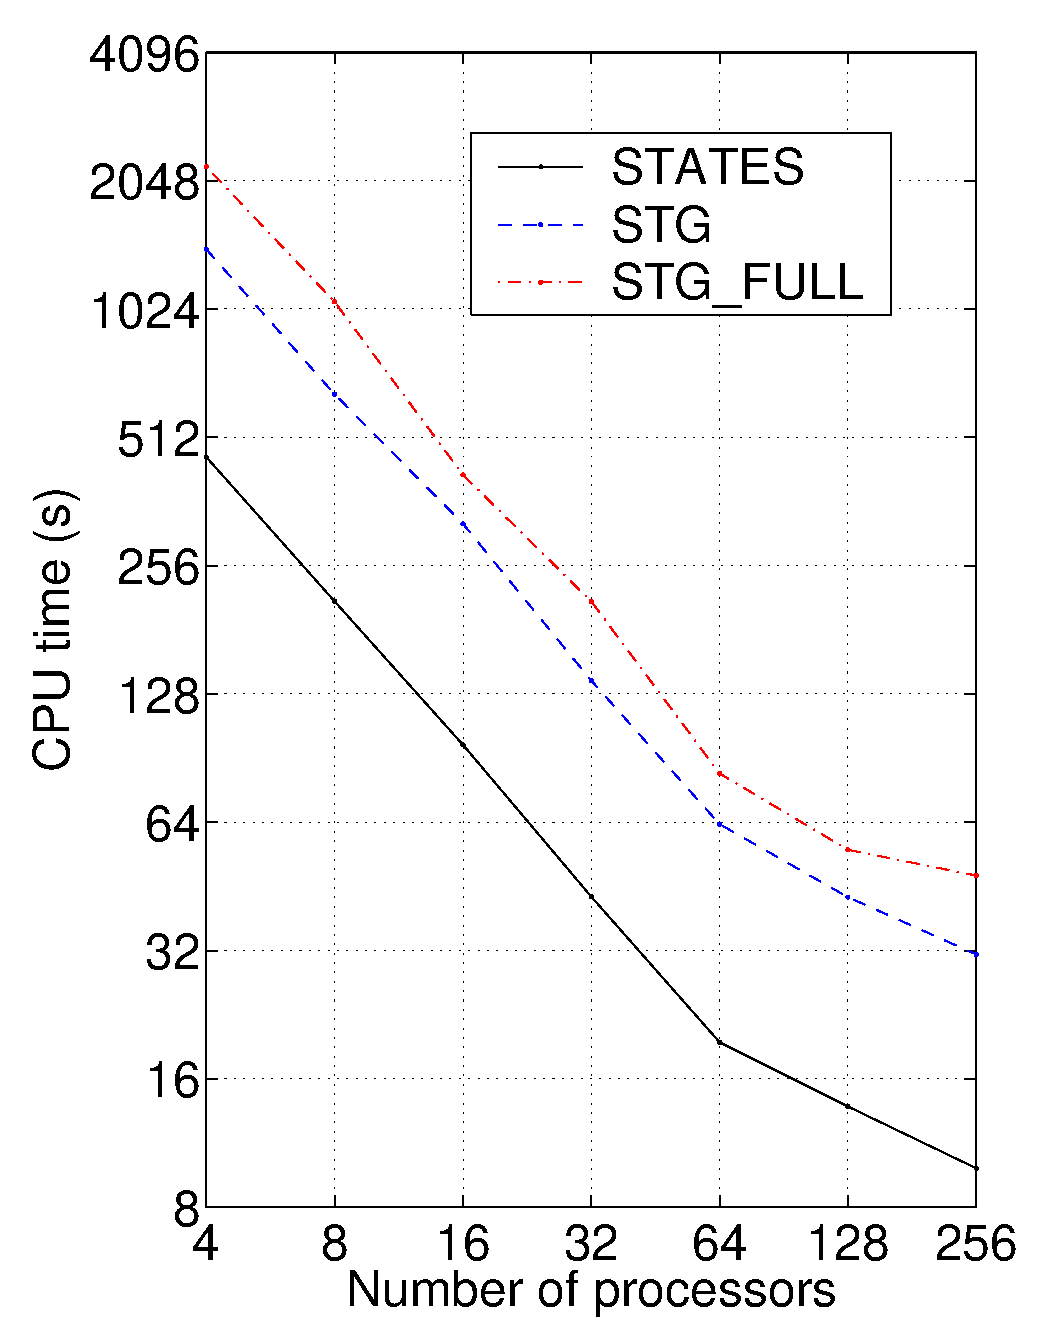
\includegraphics[width=.85\textwidth]{speedup.eps}
  \end{minipage}
  \begin{minipage}[c]{.5\textwidth}
    \centering
    \begin{tabularx}{\textwidth}{cccc}\hline
      $P$ &  STATES  &   STG   & STG\_FULL \\ \hline
      4  &  460.31  &  1414.53  & 2208.14  \\
      8  &  211.20  &   646.59  & 1064.94  \\
     16  &   97.16  &   320.78  &  417.95  \\
     32  &   42.78  &   137.51  &  210.84  \\
     64  &   19.50  &    63.34  &   83.24  \\
     128  &   13.78  &    42.71  &   55.17  \\
     256  &    9.87  &    31.33  &   47.95  \\ \hline
   \end{tabularx}
 \end{minipage}
 \figcaption{Speedup results for the integration of the state equations only
   (solid line and column 'STATES'), staggered sensitivity analysis without
   error control on the sensitivity variables (dashed line and column 'STG'),
   and staggered sensitivity analysis with full error control (dotted line and
   column 'STG\_FULL')}
 \label{f:speedup}
\end{figure}


\section{Availability}\label{s:availability}

The CVODES package has been released under a BSD open source license and is 
freely available at the web site
{\bf www.llnl.gov/CASC/sundials},
or through the DOE ACTS web site at
{\bf acts.nersc.gov/sundials/main.html}.

\section{Conclusions}\label{s:conclusions}

CVODES is the first in a series of new additions to SUNDIALS. The new codes,
IDAS and KINSOLS, together with CVODES, will provide sensitivity analysis
for all the classes of problems addressed by the basic SUNDIALS solvers.
These new capabilities extend the versatility and functionality of the SUNDIALS
solvers in addressing new classes of applications, such as dynamically-constrained
optimization, inversion, and uncertainty quantification.

Like all of SUNDIALS, CVODES is under active development.
An area of particular interest is in the automatic generation of the
sensitivity equations. A parser and code generator for the automatic
generation of derivative approximations using the complex step method
is underway.
Automatic differentiation (AD) tools will be incorporated as they
become available; we are especially interested in adding reverse AD
capabilities to the SUNDIALS adjoint sensitivity solvers.
We are currently investigating alternatives to checkpointing within
the adjoint solver in CVODES: one direction is in using reduced order
models of the forward problem, while another is in storing the
complete decision history on the first forward pass and re-using it on
the second pass.
Finally, to address language interoperability issues and thus
facilitate the use of the SUNDIALS solvers for users of other
programming languages, we plan to generate Babel~\cite{KKPR:01}
wrappers for them.
 


%=======================================================================
% Bibliography
\bibliographystyle{acmtrans}
\bibliography{../biblio}

%=======================================================================
% The article should end by the following lines. 
% The actual dates will be supplied by the Editor-in-Chief.

\begin{received}
Received Month Year;
revised Month Year; accepted Month Year
\end{received}

\end{document}
